\section{Range-metric generalization experiment}
This is a separately frozen exploratory follow-up motivated by the small total
gain of the VUS-only public consumer. It reuses all 73 recordings and 584 fixed
profiles, not a held-out dataset. No old VUS outcome is relabeled as new range
evidence. Four complete calls are compared at the 100 evenly spaced strict
thresholds used by the public range-F1 consumer: vectorized prefix/interval
recomputation, a fused compiled raster scan, the score-sorted endpoint sweep,
and query bucketing. The raster uses constant reducer workspace and no
per-threshold interval arrays; only methods requiring prefix preparation pay
for it. Thus Python-versus-compiled overhead does not explain the main comparison.
Eight cyclic/reverse orders balance four grid methods. A separate AB/BA study
compares raster and sweep over every observed distinct threshold, with two
complete eight-profile calls per method. Timings include validation, query
construction, preparation, sorting, curves and maximizing-value selection;
they exclude training and file I/O.

\begin{table*}[t]
\centering\small
\caption{Range-F1 study: case geometric speedup over the fused compiled
raster, with familywise 95\% intervals over three collections separately per
comparison. Apple rows are the original M1 Pro run; Linux rows are the
fresh combined EPYC 7763 run. Hosts and query contracts are not pooled.}
\label{tab:range-sweep}
\begin{tabular}{lrrr}
\toprule
Host / collection & Grid100 raster/bucket & Distinct raster/sweep & Distinct wins/cases\\
\midrule
Apple NAB & $1.719\ [1.625,1.814]$ & $27.80\ [18.74,41.94]$ & 20/20\\
Apple SMAP & $1.994\ [1.817,2.252]$ & $21.44\ [8.57,43.14]$ & 16/17\\
Apple SMD & $1.969\ [1.884,2.095]$ & $128.08\ [95.09,154.61]$ & 36/36\\
\midrule
Linux NAB & $1.900\ [1.616,2.239]$ & $29.35\ [18.81,46.08]$ & 20/20\\
Linux SMAP & $2.898\ [2.624,3.260]$ & $27.76\ [11.63,53.75]$ & 16/17\\
Linux SMD & $3.574\ [3.412,3.789]$ & $163.60\ [125.92,193.02]$ & 36/36\\
\bottomrule
\end{tabular}
\end{table*}

\begin{figure*}[t]
\centering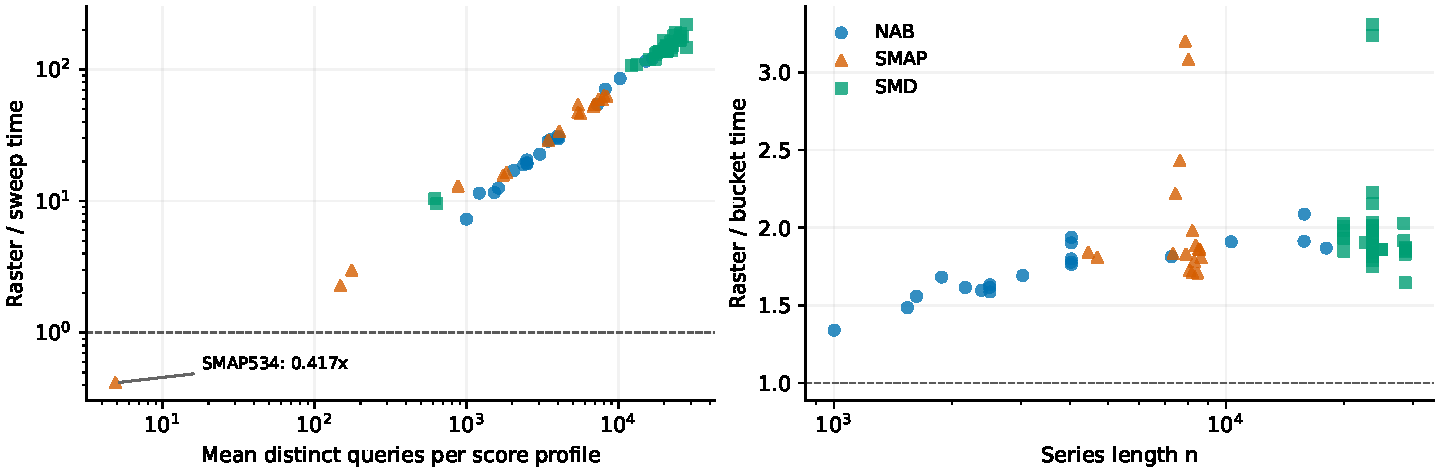
\includegraphics[width=.96\textwidth]{figures/range_sweep_cases.pdf}
\caption{All 73 original Apple range-metric cases, each with eight score profiles.
Ratios use median complete-call times against the fused compiled raster.
Left: exhaustive observed thresholds; right: the fixed 100-query contract.
The low-cardinality loss remains visible. These are descriptive fixed-panel
observations, not controlled interventions on query count or series length.}
\label{fig:range-cases}\end{figure*}

In the original Apple study, every canonical precision/recall/F1 curve is archived for every method and
profile; each repetition's output hash must match. A separate auditor imports
no metric implementation and reconstructs curve agreement, maximizing values,
thresholds, winner sets and paired intervals. Maximum reconstructed curve
discrepancy is $3.00\cdot10^{-15}$, with no cross-method model-winner-set
differences. This is numerical cross-implementation evidence, not an independent
mathematical oracle on every real input. Set-intersection oracles additionally
cover exhaustive short tied inputs and randomized boundary/query cases.

Table~\ref{tab:range-sweep} shows a clear measured algorithmic advantage over
the fused raster at exhaustive observed thresholds; Figure~\ref{fig:range-cases}
retains every case. For the 100-grid, bucketing
wins on all 73 case medians; the score-sorted sweep is 1.39/1.41/1.87 times
slower than bucketing geometrically. It wins on one SMAP case, which remains
reported. The exhaustive sweep loses on SMAP534, whose eight profiles have
only 3--11 distinct scores: raster takes 0.838\,ms versus 2.012\,ms for sweep.
Small distinct cardinality can favor scanning. For SMD, equal weighting of its
nine label blocks gives raster/sweep $112.34\ [46.21,167.79]$ and raster/bucket
$2.028\ [1.869,2.435]$; this does not establish independent physical sources.

\paragraph{What exact threshold evaluation changes.}
Holding scores, labels and $\alpha=.2$ fixed, replacing the 100-grid by observed
distinct thresholds changes 24/73 numerical winner sets. Fifteen have no
overlapping winning model; twelve incur at least .01 range-F1 regret when the
best grid-winning model is evaluated at its exhaustive optimum. Per-collection
nonoverlap counts are 6/20, 3/17 and 6/36; maximum regrets are .439, .150 and
.127. All ties use the predeclared $10^{-10}$ policy. These are oracle evaluation
and selection effects within this reused eight-profile panel, not improved
detector accuracy or a threshold that can be deployed without labels. Rank
changes from metric approximation are not a new conceptual discovery; the new
result is the exact update algorithm and its measured cost/fidelity tradeoff.
In a post-review descriptive comparison of the same recorded case medians,
exhaustive sweep still costs 2.19/2.14/3.01 times our grid100 bucket evaluator
on NAB/SMAP/SMD. The query contracts differ: this is the price of exhaustive
coverage relative to the fastest measured grid method, not a same-output
speed comparison or a prespecified endpoint.

\paragraph{Fresh combined reproduction.}
One command regenerated scores and executed the VUS primary/supplement and all
three range studies on an AMD EPYC 7763 Linux host. The frozen source and design
checks, four independent record audits and selected-cut/stress validation
passed. Complete generated arrays and curves are retained. The range result
again has maximum cross-method curve discrepancy $3.00\cdot10^{-15}$ and no
cross-method winner disagreement. Bucketing wins all 73 case medians;
SMAP534 remains the sole exhaustive-sweep loss (raster/sweep 0.661).
SMD equal-label-block raster/sweep is $146.45\ [67.70,208.30]$.
All 73 generated score matrices differ bitwise from the Mac; differences are
not uniformly small. Aggregate selection counts remain 24/15/12, but SMD188
and SMD200 exchange winner-change and nonoverlap status; maximum SMD regret
is .0797 instead of .127. These are regenerated-input results, not an isolated
CPU intervention. The same two public SMD187 calls are censored; completed
public scalar tolerances and million-point stress checks pass. A separate
range-only EPYC 9V45 execution also supports the direction and is archived,
but the combined run was selected before inspecting either timing report;
favorable hosts were not selected or pooled.

\paragraph{Public comparison and application boundary.}
Original Apple public comparisons are a separate length-selected panel: the three
shortest recordings in each collection, all eight profiles. TSB-AD range-F1
uses its 100-grid and $\alpha=.2$; TimeSeAD classic uses observed strict
thresholds and $\alpha=0$, with float32 precision/recall/F1 storage. The latter
requires a distinct numerical tolerance and is not silently treated as the
primary target. Each public call has a prospectively declared 60-second budget;
timeouts remain censored observations, not exact latencies or parity successes.
Grid calls match the public scalar within $6.67\cdot10^{-16}$; completed
TimeSeAD calls match within $5.66\cdot10^{-8}$. Descriptive public-grid speedups
are 501/272/384 geometrically on the three length-selected panels. TimeSeAD
ratios are 402/474 for NAB/SMAP; SMD181 and SMD185 take 31.96 and 37.71 seconds
versus 21.68 and 25.14 milliseconds. Both public calls for SMD187 exceed the
60-second limit; candidate calls have a 33.65-ms median, but no completed
public-output check is claimed for that recording. These public-library factors
combine algorithm and runtime differences. The fused compiled comparison in
Table~\ref{tab:range-sweep} is the evidence for an algorithmic gain.

A separate check applies unchanged TSB-AD binary-prediction range-F1 to each
of the 584 profiles at both recorded maximizing cuts. All 1,168 values agree
within $4.62\cdot10^{-16}$; this validates the value at each chosen cut, not
independent maximality over untested cuts. Three one-million-point numerical
stress inputs (alternating labels, one interval and dense tied scores), each
with 257 queries, compare all four methods. Maximum curve error is
$2.23\cdot10^{-12}$, below the predeclared $10^{-9}$ stress tolerance. This is
empirical numerical evidence, not a proof for arbitrary sequence lengths.
These operator studies do not measure a new whole-nine-metric acceleration.
Affiliation, the largest measured stage of the public consumer, remains
unchanged. The existing 1.031-fold whole-consumer result therefore remains the
only measured application-wide result in this manuscript.
